\vspace{-0.1in}
\section{NUMA-Aware Cache Management}
\label{sec:caches}
Section~\ref{sec:interconnect} showed that inter-socket bandwidth is an
important factor in achieving scalable NUMA GPU performance.
Unfortunately, because either the outgoing or incoming links must be underutilized
for us to reallocate that bandwidth to the saturated link, if both incoming and
outgoing links are saturated, dynamic link rebalancing yields minimal gains.
To improve performance in situations where dynamic link balancing is ineffective,
system designers can either increase link bandwidth, which is very expensive,
or decrease the amount of traffic that crosses the low bandwidth
communication channels. To decrease off-chip memory traffic, architects typically
turn to caches to capture locality.

\begin{figure*}[t]
    \centering
    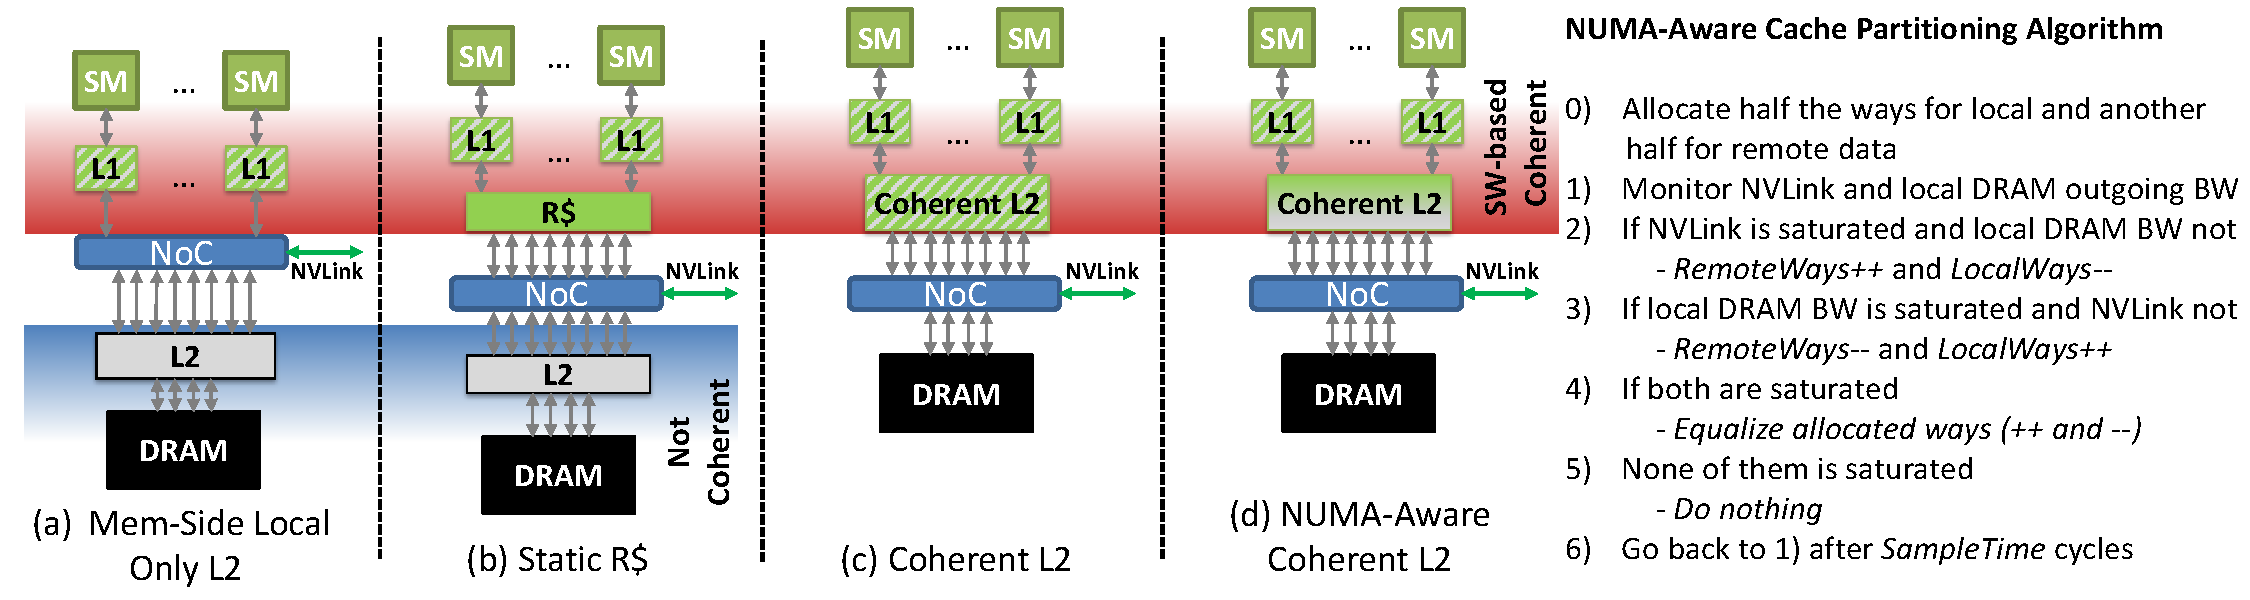
\includegraphics[width=1.0\textwidth]{figures/cache_configurations_static_dynamic.pdf}
    \caption{Potential L2 cache organizations to balance capacity between remote and
    local NUMA memory systems.}
    \label{fig:cacheorg}
            \vspace{-.1in}
\end{figure*}

GPU cache hierarchies differ from traditional CPU hierarchies as they typically do not implement strong hardware coherence protocols~\cite{singh2013cache}. 
They also differ from CPU protocols in that caches may be both processor side 
(where some form of 
coherence is typically necessary) or they may be memory side (where coherence 
is not necessary).  As described in Table~\ref{tab:setup} and
Figure~\ref{fig:cacheorg}(a), a GPU today is typically composed of relatively 
large SW managed coherent L1 caches located close to the SMs, while a relatively small, 
distributed, 
non-coherent memory side L2 cache resides close to the memory controllers.  
This organization works well for GPUs 
because their SIMT processor designs often allow for significant coalescing 
of requests to the same cache line, so having large L1 caches reduces the 
need for global crossbar bandwidth.  The memory-side L2 caches do not need to participate in the coherence protocol, which reduces a system complexity.

\vspace{-0.1in}
\subsection{Design Considerations}
In NUMA designs, remote memory references occurring across low bandwidth NUMA 
interconnections results in poor performance, as shown in 
Figure~\ref{fig:motivation}. Similarly, in NUMA GPUs utilizing
traditional memory-side L2 caches (that depend on fine grained memory 
interleaving for load balancing) is a bad decision. Because memory-side caches only
cache accesses that originate in their local memory, they cannot
cache memory from other NUMA zones and thus can not reduce NUMA interconnect traffic.  
Previous work has proposed that GPU L2 cache capacity should be split between 
memory-side caches and a new processor-side L1.5 cache that is an extension 
of the GPU L1 caches~\cite{Arunkumar2017} to enable caching of remote data, shown
in Figure~\ref{fig:cacheorg}(b). By balancing L2 capacity between memory side 
and remote caches (R\$), this design limits the need for extending expensive coherence
operations (invalidations) into the entire L2 cache while still 
minimizing crossbar or interconnect bandwidth.

\textbf{Flexibility:} Designs that statically allocate cache capacity to local memory and remote memory, 
in any balance, may achieve reasonable performance in specific instances 
but they lack flexibility. Much like application phasing was shown to affect 
NUMA bandwidth consumption the ability to dynamically share cache capacity between local and 
remote memory has the potential to improve performance under several 
situations. First, when application phasing results in some GPU-sockets
primarily accessing data locally while others are accessing data remotely,
a fix partitioning of cache capacity is guaranteed to be sub-optimal.
Second, while 
we show that most applications will be able to completely fill large 
NUMA GPUs, this may not always be the case. GPUs within the data center are 
being virtualized and there is continuous work to improve concurrent execution 
of multiple kernels and processes within a single GPU~\cite{park2015chimera, lin2016enabling, puthoor2016implementing, HSATASKMODEL}. If a large NUMA GPU is sub-partitioned, it is intuitive 
that system software attempt to partition it along the NUMA boundaries (even within
a single GPU-socket) to improve the locality of small GPU kernels.
To effectively  capture locality in these situation, NUMA-aware GPUs need to be able to 
dynamically re-purpose cache capacity at runtime, rather than be statically partitioned at design time. 

\textbf{Coherence:} To-date, discrete
single socket GPUs have not moved their memory-side caches to processor side 
because the overhead of cache invalidation (due to coherence) is an 
unnecessary performance penalty.  Within a single socket GPU with a uniform
memory system, there is little performance advantage to implementing L2 caches
as processor side caches.  However in a multi-socket NUMA design, the performance tax
of extending coherence into L2 caches is offset by the fact that remote memory
accesses can now be cached locally and may be justified;
Figure~\ref{fig:cacheorg}(c) shows a configuration with 
a coherent L2 cache where remote and local data contend for L2 capacity as
extensions of the L1 caches, implementing identical coherence policy.

\textbf{Dynamic Partitioning:} Building upon coherent GPU L2 caches, we posit that while 
conceptually simple, allowing both remote and 
local memory accesses to contend for cache capacity (in both the L1 and L2 caches) 
in a NUMA system is flawed. In UMA systems it is well know that performance 
is maximized by optimizing for cache 
hit rate, thus minimizing off-chip memory system bandwidth. However in NUMA systems, 
\textit{not all cache misses have the same relative cost
performance impact}. A cache miss to a local memory address has a 
smaller cost (in both terms of latency and bandwidth) than a cache miss to a 
remote memory address. Thus, it should be beneficial to dynamically 
skew cache allocation to preference caching remote memory over 
local data when it is determined the system is bottle-necked on NUMA bandwidth.

\begin{figure*}[t]
    \centering
    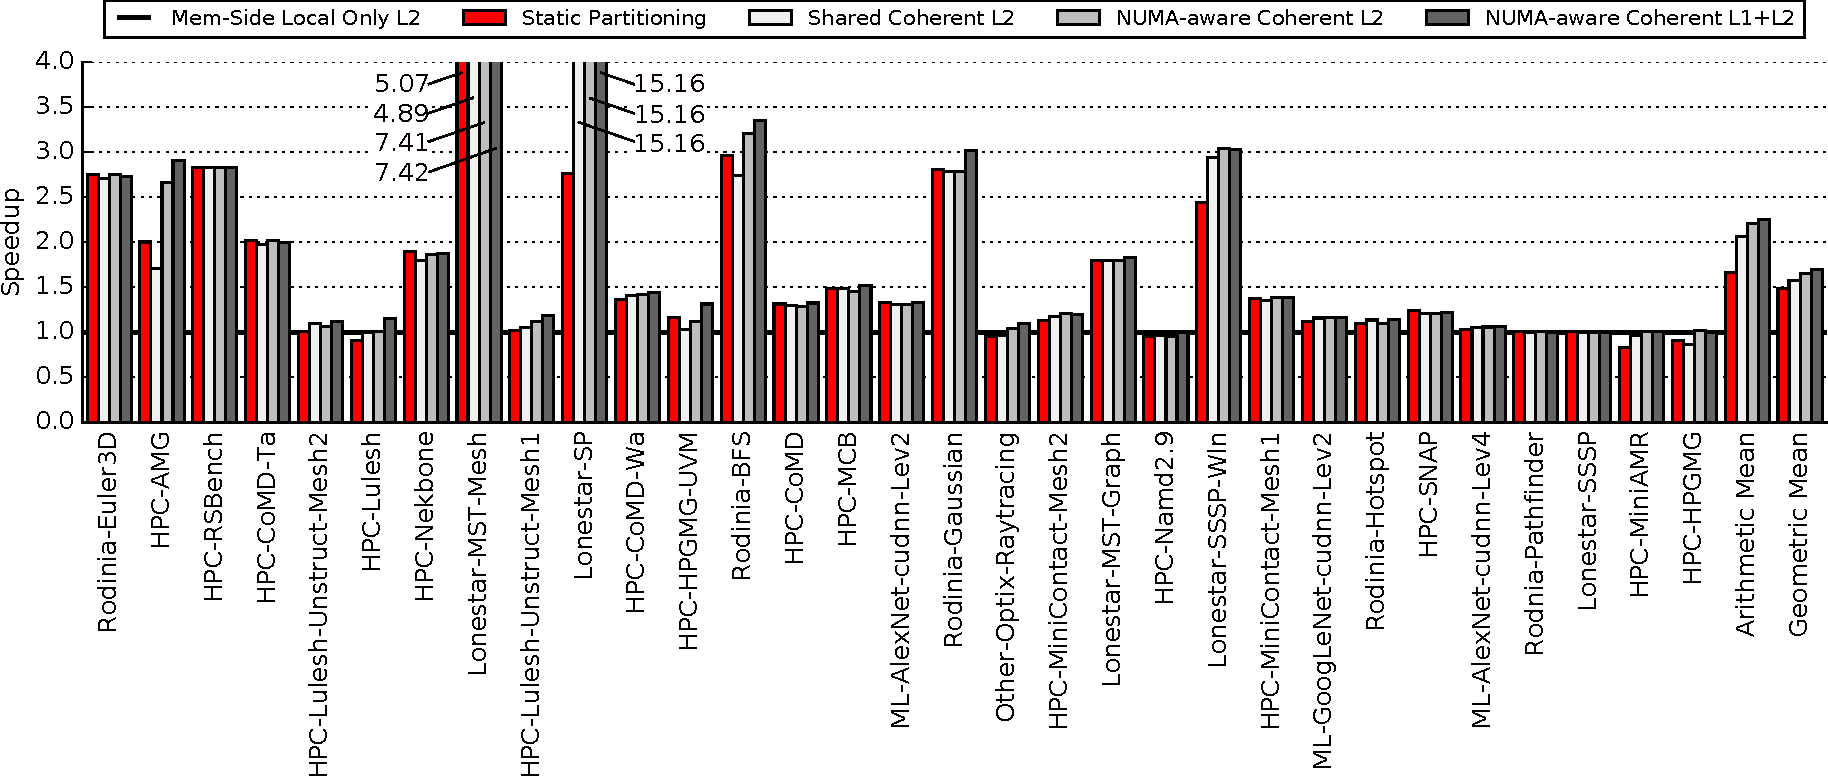
\includegraphics[width=1.0\textwidth]{figures/plot_merged_cache_WB.pdf}
    \caption{Performance of 4-socket NUMA-aware cache partitioning, compared to memory-side L2 and static partitioning.}
    \label{fig:dynamiccaching}
        \vspace{-.1in}
\end{figure*}

\begin{figure}[t]
    \centering
    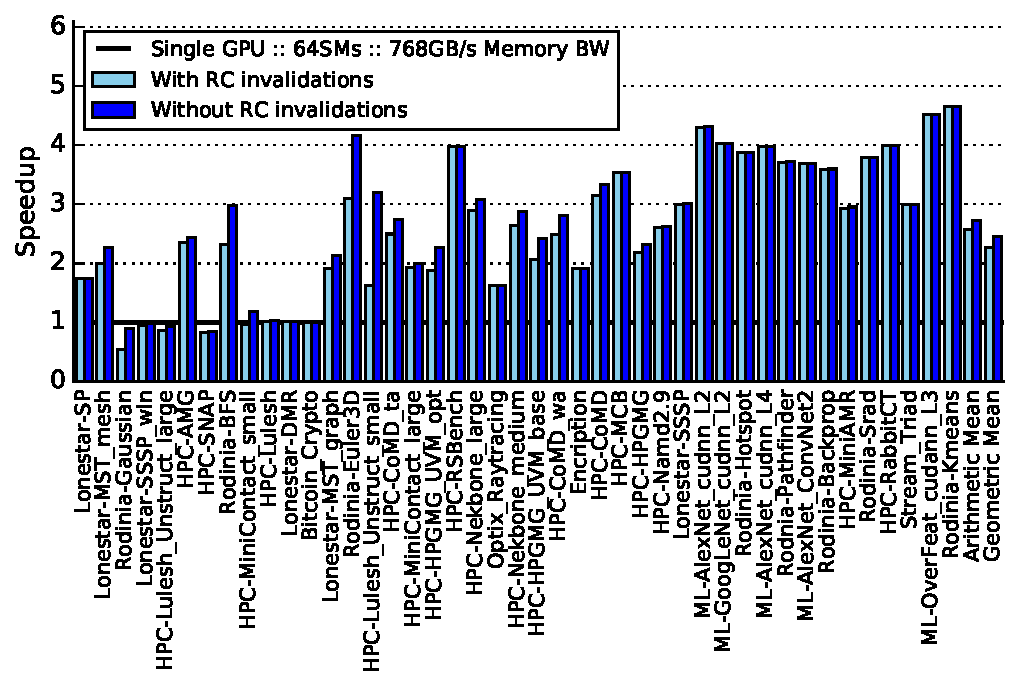
\includegraphics[width=1.0\columnwidth]{figures/plot_no_inval_WB.pdf}
     \vspace{-0.3in}
    \caption{Performance overhead of extending current GPU software based coherence
    into the GPU L2 caches.}
    \label{fig:invalidations}
    \vspace{-.1in}
\end{figure}


To minimize inter-GPU bandwidth in multi-socket GPU systems we propose a
NUMA-aware cache partitioning algorithm, with cache organization and brief summary 
shown in Figure~\ref{fig:cacheorg}(d).  Similar to our interconnect balancing
algorithm, at initial kernel launch (after GPU caches have been flushed for
coherence purposes) we allocate one half of the cache ways for local memory and 
the remaining ways for remote data (Step \circled{0}). After executing for a 5K cycles 
period, we sample the average bandwidth utilization on local memory and estimate
the GPU-socket's incoming read request rate by looking at the outgoing request rate
multiplied by the response packet size.  By using the outgoing request rate to estimate
the incoming bandwidth, we avoid situations where incoming writes may saturate
our link bandwidth falsely indicating we should preference remote data caching.
Projected link utilization above 99\% is considered to be bandwidth saturated 
(Step \circled{1}). In cases where the interconnect bandwidth is saturated but
local memory bandwidth is not, the partitioning algorithm attempts to reduce remote 
memory traffic by re-assigning one way from the group of local ways to the
remote ways grouping (Step \circled{2}).
Similarly, if the local memory BW is saturated and inter-GPU bandwidth is not, the policy 
re-allocates one way from the remote group, and allocates it to the group of local ways (Step 
\circled{3}).  To minimize the impact on cache design, all ways are consulted on look
up, allowing lazy eviction of data when the way partitioning changes.
In case where both the interconnect and local memory bandwidth 
are saturated, our policy gradually equalizes the number of ways assigned for remote 
and local cache lines (Step \circled{4}). Finally, if neither of the links are 
currently saturated, the policy takes no action (Step \circled{5}).  To prevent
cache starvation of either local or remote memory (which causes memory latency
dramatically increase and a subsequent drop in performance), we always require at 
least one way in all caches to be allocated to either remote of local memory.

\begin{figure*}[tp]
    \centering
    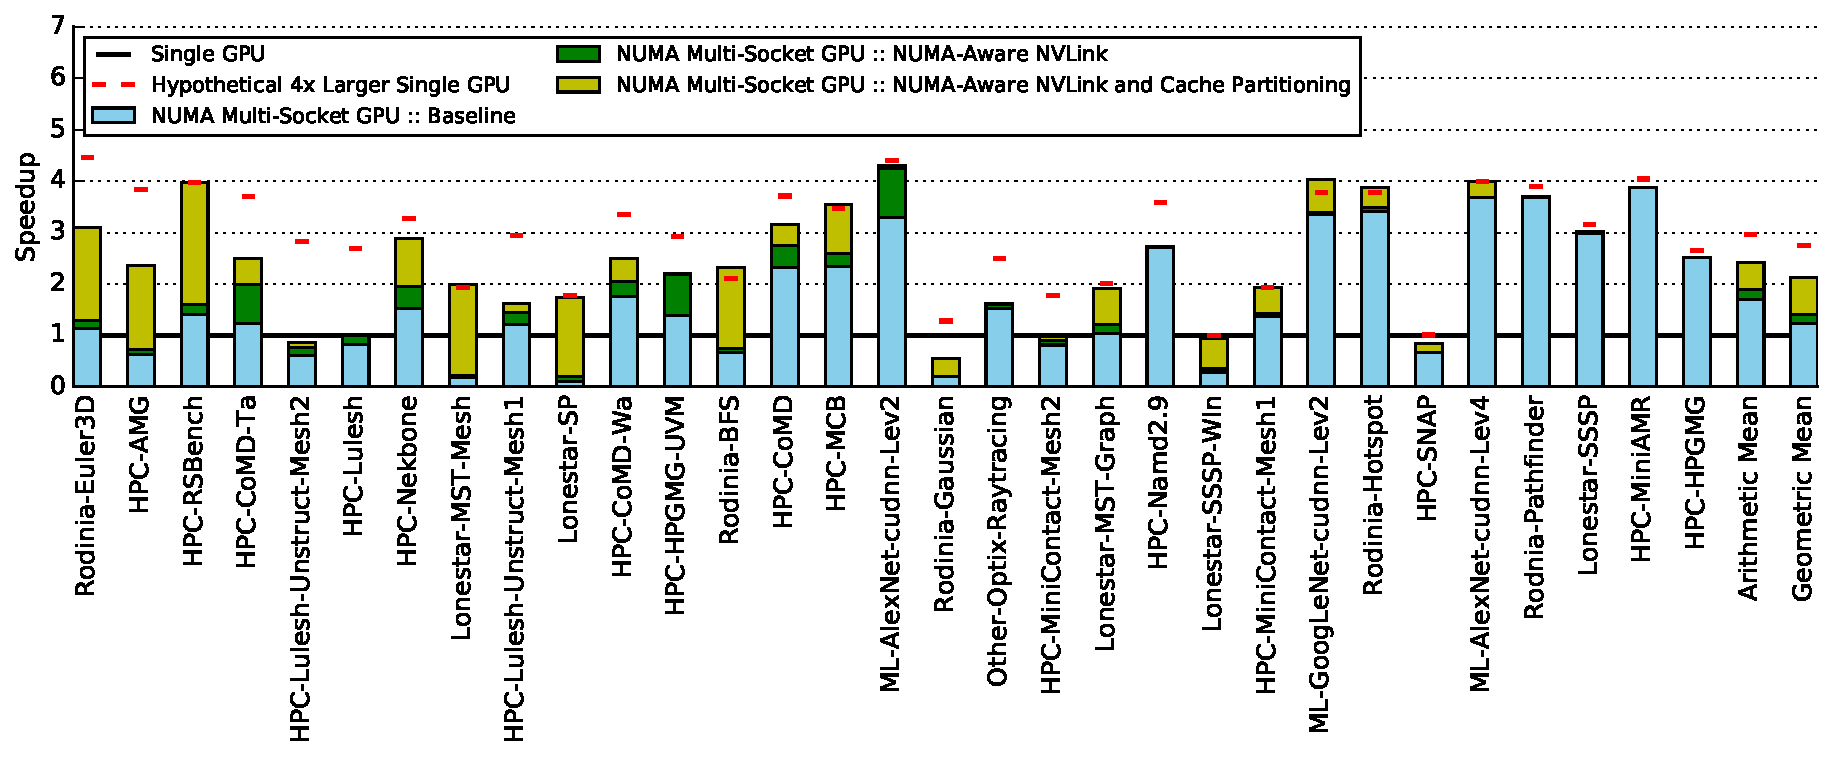
\includegraphics[width=1.0\textwidth]{figures/plot_final_speedup_WB_nvlink_first.pdf}
    \vspace{-0.2in}
    \caption{Final NUMA-aware GPU performance compared to a single GPU and 4$\times$ larger single GPU with scaled resources.}
    \label{fig:combined}
    \vspace{-.1in}
\end{figure*}

\vspace{-0.1in}
\subsection{Results}

Figure~\ref{fig:dynamiccaching} compares the performance of 4 different cache
configurations in our 4-socket NUMA GPU. Our baseline is a traditional
GPU with memory-side local-only write-back L2 caches. To compare against prior work~\cite{Arunkumar2017} we
provide a 50--50 static partitioning where the L2 cache budget is split between the 
GPU-side coherent remote cache which contains only 
remote data, and the memory side L2 which contains only local data. In our 4-socket NUMA
GPU static partitioning improves performance by 54\% on average, although for some benchmarks, 
it hurts the performance by as much as 10\% for workloads that have negligible
inter-socket memory traffic. We also show the results for GPU-side
coherent L1 and L2 caches where both local and remote data contend capacity.
On average, this solution outperforms static cache partitioning significantly
despite incurring additional flushing overhead due to cache coherence.

Finally, our proposed NUMA-aware cache 
partitioning policy is shown in dark grey. Due to its ability to
dynamically adapt the capacity of both L2 and L1 to optimize performance when backed
by NUMA memory, it is the highest performing cache configuration. By examining
simulation results we find that for workloads on the left side of Figure~\ref{fig:dynamiccaching} 
which fully saturate the inter-GPU bandwidth, NUMA-aware dynamic policy configures the L1 and 
L2 caches to be primarily used as remote caches.  However, workloads on the right 
side of the figure tend to have good GPU-socket memory locality, and thus 
prefer L1 and L2 caches store primarily local data. NUMA-aware cache
partitioning is able to flexibly adapt to varying memory access profiles and
can improve average NUMA GPU performance 76\% compared to traditional memory side L2
caches, and 22\% compared to previously proposed static cache partitioning despite
incurring additional coherence overhead.

When extending SW-controlled 
coherence into the GPU L2 
caches, L1 coherence operations must be extended into the GPU 
L2 caches. Using bulk software invalidation to maintain coherence is simple to
implement but is a performance penalty when falsely evicting
data that is not required. The overhead of this
invalidation is dependant on both the frequency of the invalidations as well as aggregate cache
capacity invalidated. Extending the L1 invalidation protocol into the large shared L2, and then across
multiple GPUs, increases both the capacity affected and frequency of the invalidation events.

To understand the impact of these invalidations, we evaluate hypothetical L2 caches which can ignore the cache 
invalidation events; thus representing
the upper limit on performance (no coherence evictions ever occur) that could be achieved by 
using a finer granularity HW-coherence protocol.
Figure~\ref{fig:invalidations} shows the impact these invalidation
operations have on application performance.
While significant for
some applications, on average SW-based cache invalidations overheads are only 10\%, even
when extended across all GPU-socket L2 caches.  So while fine grain HW coherence protocols
may improve performance, the magnitude of their improvement must be weighted against their
hardware implementation complexity. While in the studies above we assumed a write-back policy in L2 caches, as a sensitivity study we also evaluated the effect of using a write-through cache policy to mirror the write-through L1 cache policy. Our findings indicate that write-back L2 outperforms write-through L2 by 9\% on average in our NUMA-GPU design due to the decrease in total inter-GPU write bandwidth.





